%==============================================================================
%  EECS 370 — Introduction to Computer Organization
%  THE COMPLETE OPEN-BOOK EXAM CHEAT SHEET
%
%  Designed to teach the entire course from zero: every topic is explained
%  from first principles with worked examples and diagrams, so that a reader
%  who never attended a single lecture can solve exam problems.
%
%  Compile with:  pdflatex eecs370-cheatsheet.tex   (run twice for refs/TOC)
%==============================================================================
\documentclass[10pt]{article}

% ---------- Packages ----------
\usepackage[margin=0.7in]{geometry}
\usepackage[T1]{fontenc}
\usepackage{lmodern}
\usepackage{amsmath,amssymb}
\usepackage{xcolor}
\usepackage{tikz}
\usetikzlibrary{shapes.geometric,arrows.meta,positioning,fit,calc,backgrounds,matrix,decorations.pathreplacing}
\usepackage{tcolorbox}
\tcbuselibrary{skins,breakable}
\usepackage{enumitem}
\usepackage{booktabs}
\usepackage{array}
\usepackage{multicol}
\usepackage{listings}
\usepackage[explicit]{titlesec}
\usepackage{fancyhdr}
\usepackage{hyperref}

% ---------- Colors ----------
\definecolor{maize}{RGB}{255,203,5}      % Michigan Maize
\definecolor{umblue}{RGB}{0,39,76}       % Michigan Blue
\definecolor{accent}{RGB}{0,93,135}
\definecolor{soft}{RGB}{236,243,248}
\definecolor{codebg}{RGB}{245,245,238}
\definecolor{good}{RGB}{0,120,70}
\definecolor{warn}{RGB}{176,0,32}
\definecolor{gridline}{RGB}{170,170,170}

\hypersetup{colorlinks=true, linkcolor=umblue, urlcolor=accent,
  pdftitle={EECS 370 Complete Cheat Sheet}, pdfauthor={EECS 370}}

% ---------- Section styling ----------
\titleformat{\section}
  {\normalfont\Large\bfseries}
  {}{0pt}
  {\colorbox{umblue}{\parbox{\dimexpr\textwidth-2\fboxsep}{\strut\color{white}\thesection\quad#1}}}
\titleformat{\subsection}
  {\normalfont\large\bfseries\color{umblue}}{}{0pt}
  {\thesubsection\quad#1}
  [{\color{maize}\titlerule[2pt]}]
\titleformat{\subsubsection}
  {\normalfont\bfseries\color{accent}}{}{0pt}{#1}

% ---------- Header / Footer ----------
\pagestyle{fancy}
\fancyhf{}
\renewcommand{\headrulewidth}{1pt}
\renewcommand{\headrule}{\hbox to\headwidth{\color{maize}\leaders\hrule height \headrulewidth\hfill}}
\lhead{\small\color{umblue}\textbf{EECS 370} — Computer Organization}
\rhead{\small\color{umblue}Open-Book Exam Cheat Sheet}
\cfoot{\small\color{umblue}\thepage}

% ---------- Boxes ----------
\newtcolorbox{keybox}[1][Key Idea]{
  colback=soft, colframe=umblue, fonttitle=\bfseries\color{white},
  coltitle=white, title=#1, boxrule=0.8pt, arc=2pt, left=4pt,right=4pt,
  top=2pt,bottom=2pt, breakable}
\newtcolorbox{formbox}[1][Formula]{
  colback=maize!18, colframe=umblue!80, fonttitle=\bfseries,
  title=#1, boxrule=0.8pt, arc=2pt, left=4pt,right=4pt,top=2pt,bottom=2pt, breakable}
\newtcolorbox{tipbox}[1][Exam Tip]{
  colback=good!8, colframe=good, fonttitle=\bfseries\color{white},
  coltitle=white, title=#1, boxrule=0.8pt, arc=2pt,left=4pt,right=4pt,top=2pt,bottom=2pt, breakable}
\newtcolorbox{pitbox}[1][Common Mistake]{
  colback=warn!7, colframe=warn, fonttitle=\bfseries\color{white},
  coltitle=white, title=#1, boxrule=0.8pt, arc=2pt,left=4pt,right=4pt,top=2pt,bottom=2pt, breakable}

% ---------- Code listing style ----------
\lstdefinestyle{asm}{
  backgroundcolor=\color{codebg}, basicstyle=\ttfamily\small,
  frame=single, framerule=0.4pt, rulecolor=\color{gridline},
  breaklines=true, columns=fullflexible, keepspaces=true,
  showstringspaces=false, xleftmargin=4pt, xrightmargin=2pt,
  commentstyle=\color{good}\itshape, keywordstyle=\color{warn}\bfseries,
  morecomment=[l]{//}, morecomment=[l]{\#}}
\lstset{style=asm}
\newcommand{\code}[1]{\texttt{\small #1}}

% ---------- Bit-field diagram macro ----------
% \bitfield{ {width/label/bits} ... }  width in cm-units
\newcommand{\bitrow}[1]{%
\begin{tikzpicture}[font=\footnotesize]
  \foreach \w/\lbl/\bits [count=\i from 0, evaluate=\i as \prev using {\i}] in {#1}{}
\end{tikzpicture}}

\setlength{\parindent}{0pt}
\setlength{\parskip}{4pt}
\setlist{leftmargin=1.3em,itemsep=1pt,topsep=2pt}

%==============================================================================
\begin{document}

% ---------------- TITLE ----------------
\begin{titlepage}
\centering
\vspace*{1.2cm}
{\color{umblue}\rule{\textwidth}{4pt}}\\[0.5cm]
{\Huge\bfseries\color{umblue} EECS 370}\\[0.3cm]
{\LARGE\bfseries\color{accent} Introduction to Computer Organization}\\[0.5cm]
{\Large The Complete Open-Book Exam Cheat Sheet}\\[0.3cm]
{\large\itshape Everything from binary to virtual memory --- taught from scratch}\\[0.4cm]
{\color{maize}\rule{\textwidth}{4pt}}\\[1cm]

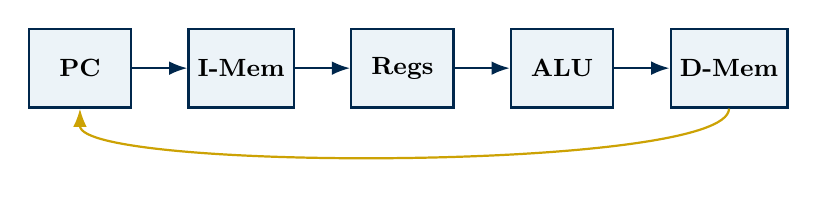
\begin{tikzpicture}
  % A tiny stylized datapath as cover art
  \tikzset{blk/.style={draw=umblue,thick,fill=soft,minimum height=1cm,minimum width=1.3cm,font=\small\bfseries}}
  \node[blk] (pc) {PC};
  \node[blk,right=0.7cm of pc] (im) {I-Mem};
  \node[blk,right=0.7cm of im] (rf) {Regs};
  \node[blk,right=0.7cm of rf] (alu) {ALU};
  \node[blk,right=0.7cm of alu] (dm) {D-Mem};
  \draw[-{Latex},thick,umblue] (pc)--(im); \draw[-{Latex},thick,umblue](im)--(rf);
  \draw[-{Latex},thick,umblue](rf)--(alu); \draw[-{Latex},thick,umblue](alu)--(dm);
  \draw[-{Latex},thick,maize!80!black] (dm.south) .. controls +(0,-0.8) and +(0,-0.8) .. (pc.south);
\end{tikzpicture}

\vfill
{\large This guide covers: number representation $\cdot$ the LC2K \& ARM/LEGv8 ISAs $\cdot$
assembly \& C translation $\cdot$ assemblers, linkers \& loaders $\cdot$ calling conventions \&
the stack $\cdot$ digital logic \& FSMs $\cdot$ single-/multi-cycle \& pipelined datapaths $\cdot$
hazards \& forwarding $\cdot$ performance \& Amdahl's Law $\cdot$ caches \& AMAT $\cdot$ virtual memory \& TLBs.}
\vfill
{\small\itshape Built as a teaching reference. Verify exact bit layouts against the official
LC2K spec on the course site before the exam.}
\end{titlepage}

\tableofcontents
\newpage

%==============================================================================
\section{Big Picture: What This Course Is About}
%==============================================================================

\begin{keybox}[The One-Sentence Summary]
EECS 370 explains \textbf{how a program written in C becomes electrons moving through
transistors}: C $\to$ assembly $\to$ machine code $\to$ executed by a datapath built from
logic gates, while a memory hierarchy (registers $\to$ cache $\to$ RAM $\to$ disk via virtual
memory) feeds it data fast enough to matter.
\end{keybox}

The course is a vertical slice through the computing stack. Read this as a pipeline:

\begin{center}
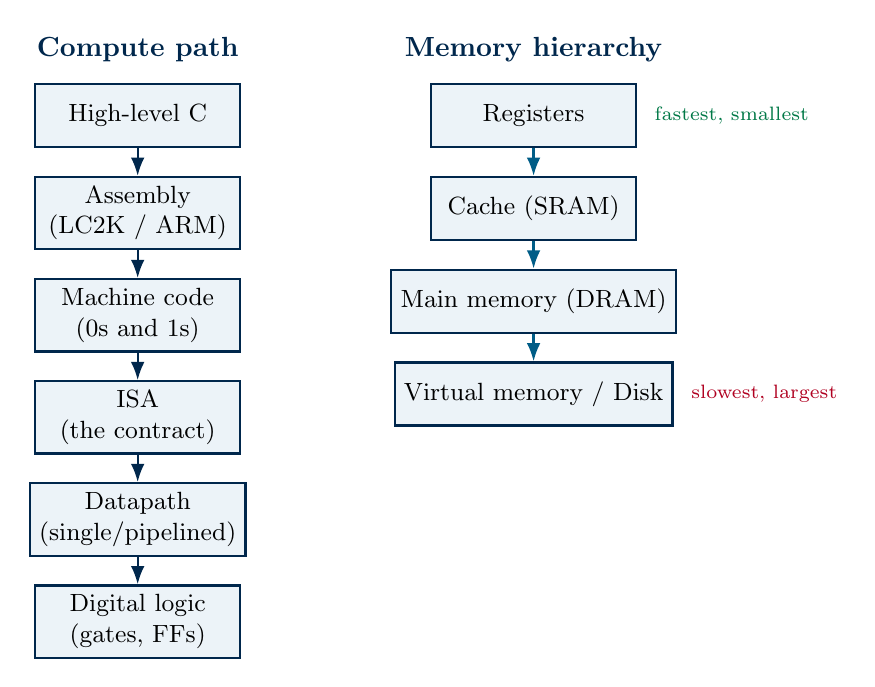
\begin{tikzpicture}[font=\small,node distance=0.35cm]
\tikzset{lay/.style={draw=umblue,thick,fill=soft,minimum width=2.6cm,minimum height=0.8cm,align=center,font=\small}}
\node[lay] (c) {High-level C};
\node[lay,below=of c] (asm) {Assembly\\(LC2K / ARM)};
\node[lay,below=of asm] (mc) {Machine code\\(0s and 1s)};
\node[lay,below=of mc] (isa) {ISA\\(the contract)};
\node[lay,below=of isa] (dp) {Datapath\\(single/pipelined)};
\node[lay,below=of dp] (lg) {Digital logic\\(gates, FFs)};
\node[lay,right=2.4cm of c] (mem1) {Registers};
\node[lay,below=of mem1] (mem2) {Cache (SRAM)};
\node[lay,below=of mem2] (mem3) {Main memory (DRAM)};
\node[lay,below=of mem3] (mem4) {Virtual memory / Disk};
\node[above=0.15cm of c,font=\bfseries\color{umblue}] {Compute path};
\node[above=0.15cm of mem1,font=\bfseries\color{umblue}] {Memory hierarchy};
\foreach \a/\b in {c/asm,asm/mc,mc/isa,isa/dp,dp/lg} \draw[-{Latex},umblue,thick] (\a)--(\b);
\foreach \a/\b in {mem1/mem2,mem2/mem3,mem3/mem4} \draw[-{Latex},accent,thick] (\a)--(\b);
\node[right=0.1cm of mem1,font=\scriptsize\color{good}] {fastest, smallest};
\node[right=0.1cm of mem4,font=\scriptsize\color{warn}] {slowest, largest};
\end{tikzpicture}
\end{center}

\begin{tipbox}[How to use this sheet in the exam]
Each topic has a \textbf{procedure} (numbered steps you can follow mechanically) plus the
\textbf{formula} and a \textbf{worked example}. On a timed exam, find the matching procedure,
plug in numbers, and check against the "Common Mistake" boxes.
\end{tipbox}

%==============================================================================
\section{Number Representation \& Binary Arithmetic}
%==============================================================================

\subsection{Positional notation and bases}
A number in base $b$ with digits $d_{n-1}\dots d_1 d_0$ has value $\sum d_i b^i$.
We use \textbf{binary} (base 2), \textbf{hex} (base 16, digits 0--9,A--F), and decimal.

\begin{formbox}[Conversions you must do instantly]
\begin{itemize}
\item \textbf{Bin$\to$Hex:} group bits into 4s from the right; each group is one hex digit.
\item \textbf{Hex$\to$Bin:} expand each hex digit to 4 bits ($\text{A}=1010$, $\text{F}=1111$).
\item \textbf{$n$ bits} represent $2^n$ distinct values.
\item \textbf{Powers:} $2^{10}=1024\approx 10^3$ (Ki), $2^{20}$ (Mi), $2^{30}$ (Gi).
\end{itemize}
\end{formbox}

\subsection{Unsigned vs. signed (two's complement)}
With $n$ bits:
\begin{itemize}
\item \textbf{Unsigned} range: $0$ to $2^n-1$.
\item \textbf{Two's complement (signed)} range: $-2^{n-1}$ to $2^{n-1}-1$. The MSB has weight
$-2^{n-1}$; all other bits have their normal positive weight.
\end{itemize}

\begin{center}
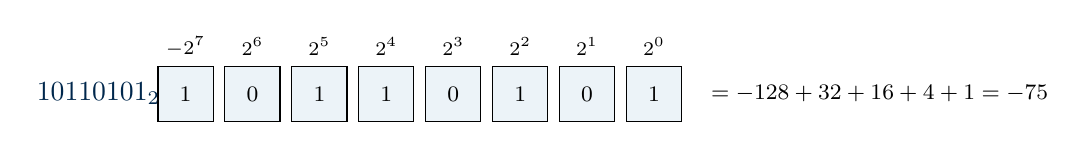
\begin{tikzpicture}[font=\footnotesize]
\foreach \b/\w [count=\i from 0] in {1/{-2^7},0/{2^6},1/{2^5},1/{2^4},0/{2^3},1/{2^2},0/{2^1},1/{2^0}}{
  \node[draw,minimum size=0.7cm,fill=soft] (c\i) at (\i*0.85,0) {\b};
  \node[font=\scriptsize] at (\i*0.85,0.6) {$\w$};
}
\node[anchor=west] at (7*0.85+0.6,0) {$=-128+32+16+4+1=-75$};
\node[anchor=east,font=\bfseries\color{umblue}] at (-0.2,0) {$10110101_2$};
\end{tikzpicture}
\end{center}

\begin{keybox}[Negate in two's complement: ``flip and add 1'']
To compute $-x$: invert every bit (one's complement), then add 1.
Example with 8 bits: $x=5=00000101$. Flip $\to 11111010$, $+1 \to 11111011 = -5$.
\textbf{Check:} $x + (-x)$ should be $0$ (with the carry-out discarded).
\end{keybox}

\subsection{Sign extension}
To widen a signed number to more bits, \textbf{copy the sign bit} into all new high bits
($0111\to 00000111$; $1011\to 11111011$). For unsigned, pad with zeros. This is why the
LC2K \code{lw/sw/beq} offset (16 bits) is \emph{sign-extended} to 32 bits before use.

\subsection{Addition, overflow, and carry}
Add like decimal but carry at 2. Two's-complement add/subtract use the \emph{same} hardware.
\begin{itemize}
\item \textbf{Unsigned overflow} = carry-out of the MSB.
\item \textbf{Signed overflow} = carry-\emph{into} MSB $\neq$ carry-\emph{out} of MSB.
Equivalently: $(+) + (+) = (-)$ or $(-) + (-) = (+)$. Adding opposite signs \emph{never} overflows.
\end{itemize}

\begin{pitbox}
``The number is negative'' $\neq$ ``overflow occurred.'' Overflow means the \emph{true} result
doesn't fit in $n$ bits. Always reason about the sign-bit rule, not just the result's sign.
\end{pitbox}

%==============================================================================
\section{Instruction Set Architecture (ISA) Fundamentals}
%==============================================================================

\begin{keybox}[What an ISA is]
The ISA is the \textbf{contract between hardware and software}: the set of instructions, the
registers, the memory model, and the binary encoding. Software targets the ISA; any hardware
that implements the ISA correctly will run that software. It is the boundary that lets one
program run on many chip generations.
\end{keybox}

\textbf{Key ISA design axes:}
\begin{itemize}
\item \textbf{RISC vs. CISC:} RISC (LC2K, ARM, MIPS) = few, simple, fixed-length instructions,
load/store architecture. CISC (x86) = many complex variable-length instructions.
\item \textbf{Load/store architecture:} ALU operations work only on registers; memory is touched
\emph{only} by load (\code{lw}) and store (\code{sw}). LC2K and ARM are load/store.
\item \textbf{Word size:} LC2K uses 32-bit words and is \textbf{word-addressed} (address $i$ =
the $i$-th word). Most real machines (ARM) are \textbf{byte-addressed}.
\item \textbf{Endianness:} byte order of a multi-byte word. Little-endian stores the
least-significant byte at the lowest address; big-endian the reverse.
\end{itemize}

%==============================================================================
\section{The LC2K ISA (Project 1 core)}
%==============================================================================

\begin{keybox}[LC2K at a glance]
\textbf{8} general registers (\code{r0}--\code{r7}), each \textbf{32 bits}. \code{r0} is an
ordinary register but conventionally holds \textbf{0} (the assembler does \emph{not} force it).
Memory is an array of \textbf{32-bit words}, \textbf{word-addressed}. Every instruction is
\textbf{one 32-bit word}. There are exactly \textbf{8 instructions} in \textbf{4 formats}.
\end{keybox}

\subsection{Instruction formats and the exact bit layout}
Bits are numbered 31 (MSB) down to 0 (LSB). The opcode is always bits \textbf{24--22}.

\newcommand{\bitcell}[3]{% x-start, width(in cells), label
}
% Helper to draw a field block: \field{xstart}{xend}{toplabel}{bottomlabel}
\newcommand{\field}[4]{%
  \draw[fill=#4] (#1,0) rectangle (#2,0.9);
  \node at ({(#1+#2)/2},0.45) {\strut #3};
}

\begin{center}
\textbf{R-type} \quad(\code{add}, \code{nor})\\[2pt]
\begin{tikzpicture}[font=\footnotesize,scale=0.95]
\field{0}{2}{unused (31--25)}{soft}
\field{2}{4}{opcode (24--22)}{maize!40}
\field{4}{6}{regA (21--19)}{accent!20}
\field{6}{8}{regB (18--16)}{accent!20}
\field{8}{11}{unused, =0 (15--3)}{soft}
\field{11}{13}{destReg (2--0)}{good!25}
\node[font=\scriptsize] at (1,1.15) {7 bits}; \node[font=\scriptsize] at (3,1.15){3};
\node[font=\scriptsize] at (5,1.15){3}; \node[font=\scriptsize] at (7,1.15){3};
\node[font=\scriptsize] at (9.5,1.15){13}; \node[font=\scriptsize] at (12,1.15){3};
\end{tikzpicture}
\end{center}

\begin{center}
\textbf{I-type} \quad(\code{lw}, \code{sw}, \code{beq})\\[2pt]
\begin{tikzpicture}[font=\footnotesize,scale=0.95]
\field{0}{2}{unused (31--25)}{soft}
\field{2}{4}{opcode (24--22)}{maize!40}
\field{4}{6}{regA (21--19)}{accent!20}
\field{6}{8}{regB (18--16)}{accent!20}
\field{8}{13}{offsetField --- 16-bit two's complement (15--0)}{warn!18}
\end{tikzpicture}\\[2pt]
{\footnotesize offsetField range $-32768$ to $+32767$; \textbf{sign-extended} to 32 bits at runtime.}
\end{center}

\begin{center}
\textbf{J-type} \quad(\code{jalr})\hfill\textbf{O-type}\quad(\code{halt}, \code{noop})\\[2pt]
\begin{tikzpicture}[font=\footnotesize,scale=0.95]
\field{0}{2}{unused}{soft}
\field{2}{4}{opcode}{maize!40}
\field{4}{6}{regA}{accent!20}
\field{6}{8}{regB}{accent!20}
\field{8}{11}{unused =0}{soft}
% O-type
\begin{scope}[xshift=12cm]
\field{0}{2}{unused}{soft}
\field{2}{4}{opcode}{maize!40}
\field{4}{8}{unused (all 0)}{soft}
\end{scope}
\end{tikzpicture}
\end{center}

\subsection{The 8 instructions (memorize this table)}
\begin{center}
\renewcommand{\arraystretch}{1.25}
\begin{tabular}{@{}l c c l l@{}}
\toprule
\textbf{Instr} & \textbf{Opcode} & \textbf{Type} & \textbf{Assembly} & \textbf{Action (RTL)}\\
\midrule
\code{add}  & 000 (0) & R & \code{add rA rB rDest}  & \code{reg[Dest] = reg[A] + reg[B]}\\
\code{nor}  & 001 (1) & R & \code{nor rA rB rDest}  & \code{reg[Dest] = \~{}(reg[A] | reg[B])}\\
\code{lw}   & 010 (2) & I & \code{lw rA rB off}     & \code{reg[B] = mem[reg[A] + off]}\\
\code{sw}   & 011 (3) & I & \code{sw rA rB off}     & \code{mem[reg[A] + off] = reg[B]}\\
\code{beq}  & 100 (4) & I & \code{beq rA rB off}    & \code{if(reg[A]==reg[B]) PC=PC+1+off}\\
\code{jalr} & 101 (5) & J & \code{jalr rA rB}       & \code{reg[B]=PC+1; PC=reg[A]}\\
\code{halt} & 110 (6) & O & \code{halt}             & increment PC, then stop machine\\
\code{noop} & 111 (7) & O & \code{noop}             & do nothing (PC$\,$++)\\
\bottomrule
\end{tabular}
\end{center}

\begin{keybox}[The two ``gotchas'' everyone trips on]
\textbf{1. \code{beq} target is PC-relative and PC is \emph{already incremented}:} target $=$
(address of the \code{beq}) $+\,1\,+\,$offset. So offset $=$ (target address) $-$ (beq address) $-1$.\\
\textbf{2. \code{jalr} edge case:} if \code{regA == regB}, the spec says \code{reg[B]} is first
written with PC+1 and then PC takes the \emph{new} value of that register --- read the spec
carefully; the link write happens before the jump uses regA.
\end{keybox}

\subsection{Building everything from 8 instructions}
LC2K is deliberately minimal --- you synthesize the rest:
\begin{itemize}
\item \textbf{Load a constant} (no ``addi''): put the value in memory with \code{.fill} and
\code{lw} it, or build it from \code{r0}.
\item \textbf{NOT x:} \code{nor x x dest} ($\overline{x|x}=\overline{x}$).
\item \textbf{Move / copy:} \code{add src r0 dest} (assuming \code{r0=0}).
\item \textbf{Subtract:} negate then add. To get $-y$: \code{nor y y t} then add a known $1$
(two's complement), or use \code{.fill} constants.
\item \textbf{Unconditional jump:} \code{beq r0 r0 off} (always taken).
\item \textbf{AND} via De Morgan: $a\,\&\,b = \overline{\overline{a}\mid\overline{b}}$ using three \code{nor}s.
\end{itemize}

%==============================================================================
\section{LC2K Assembly, the Assembler, Linker \& Loader}
%==============================================================================

\subsection{Assembly source format}
Each line: \code{[label]\quad opcode\quad field0 field1 field2\quad \# comment}.
Labels start in column 1 (max 6 chars, begin with a letter). Fields are decimal numbers
\emph{or} labels (for the offset/address fields).

\begin{lstlisting}
        lw      0  1  five     // reg1 = mem[five] = 5
        lw      0  2  neg1     // reg2 = -1
start   add     1  2  1        // reg1 = reg1 + reg2  (count down)
        beq     0  1  done     // if reg1==0 goto done (reg0 is 0)
        beq     0  0  start     // unconditional jump back
done    halt
five    .fill   5
neg1    .fill   -1
stk     .fill   0
\end{lstlisting}

\begin{keybox}[The \code{.fill} directive]
\code{.fill N} places the 32-bit value \code{N} into the next memory word. \code{N} may be a
number \emph{or a label} --- if it's a label, the assembler stores that label's \emph{address}.
This is how you make constants, jump tables, and pointers. \code{.fill} is \emph{not} an
instruction; it's data placed inline in the program image.
\end{keybox}

\subsection{Two-pass assembler}
\begin{enumerate}
\item \textbf{Pass 1 --- build the symbol table.} Walk every line, tracking the address (line
number, since each line is one word). Record each \texttt{label $\to$ address}. Catch duplicate labels.
\item \textbf{Pass 2 --- generate machine code.} For each line, look up any label operands in the
symbol table, compute offsets (for \code{beq}: \code{labelAddr - (PC+1)}), assemble the 32-bit
word, and emit it as a decimal integer (one per line).
\end{enumerate}

\begin{tipbox}[Why two passes?]
\textbf{Forward references.} A \code{beq} can jump to a label defined later in the file. You
cannot fill in its offset until you know that label's address, so pass 1 finds all addresses
first, then pass 2 resolves them.
\end{tipbox}

\subsection{Linker: combining multiple files}
Real programs are split across files compiled separately. The linker stitches them together.
\begin{itemize}
\item \textbf{Global labels:} a label is global if it's referenced across files. Two label kinds
in object files:
  \begin{itemize}
  \item \textbf{Defined (Symbol Table):} ``I provide label \code{X} at offset $k$ in my text/data.''
  \item \textbf{Undefined (Relocation Table):} ``I use label \code{Y} but don't define it --- patch me.''
  \end{itemize}
\item \textbf{Relocation:} when files are concatenated, every absolute address (e.g. a
\code{.fill label} or an \code{lw/sw} that uses a label) must be \emph{relocated} by adding the
base offset of its section. PC-relative \code{beq} offsets do \emph{not} need relocation (they
are self-relative within the file). This is exactly Project~2's linker logic.
\item \textbf{Loader:} copies the final image into memory at its load address and starts execution
at the entry point.
\end{itemize}

\begin{center}
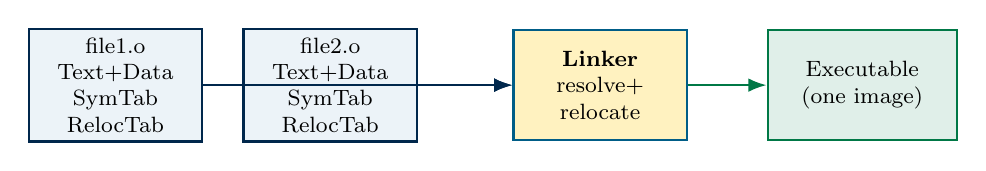
\begin{tikzpicture}[font=\footnotesize,node distance=0.5cm]
\tikzset{f/.style={draw=umblue,thick,fill=soft,minimum width=2.2cm,minimum height=1.4cm,align=center}}
\node[f] (a) {file1.o\\Text+Data\\SymTab\\RelocTab};
\node[f,right=of a] (b) {file2.o\\Text+Data\\SymTab\\RelocTab};
\node[draw=accent,thick,fill=maize!25,minimum width=2.2cm,minimum height=1.4cm,right=1.2cm of b,align=center] (l) {\textbf{Linker}\\resolve+\\relocate};
\node[draw=good,thick,fill=good!12,minimum width=2.4cm,minimum height=1.4cm,right=1.0cm of l,align=center] (e) {Executable\\(one image)};
\draw[-{Latex},umblue,thick] (a)--(l); \draw[-{Latex},umblue,thick] (b)--(l);
\draw[-{Latex},good,thick] (l)--(e);
\end{tikzpicture}
\end{center}

%==============================================================================
\section{The ARM / LEGv8 ISA}
%==============================================================================

\begin{keybox}[Why ARM too?]
LC2K teaches the bare minimum; ARM (the LEGv8 teaching subset from Patterson \& Hennessy) shows a
real, byte-addressed, 64-bit RISC ISA with a richer instruction set and a real calling convention.
\end{keybox}

\subsection{Registers}
32 registers, 64 bits each: \code{X0}--\code{X30} plus \code{XZR} (the zero register, reads 0).
\begin{center}
\renewcommand{\arraystretch}{1.15}
\begin{tabular}{@{}l l l@{}}
\toprule
\textbf{Register} & \textbf{Role} & \textbf{Saved by}\\
\midrule
\code{X0--X7}   & arguments / return values         & caller-saved\\
\code{X8}       & indirect result location          & ---\\
\code{X9--X15}  & temporaries                       & caller-saved\\
\code{X16--X17} & scratch (IP0/IP1)                 & caller-saved\\
\code{X18}      & platform register                 & ---\\
\code{X19--X27} & saved registers                   & callee-saved\\
\code{X28 (SP)} & stack pointer                     & callee-saved\\
\code{X29 (FP)} & frame pointer                     & callee-saved\\
\code{X30 (LR)} & link register (return address)    & callee-saved\\
\code{XZR}      & constant zero                     & ---\\
\bottomrule
\end{tabular}
\end{center}

\subsection{Core instructions}
\begin{center}
\renewcommand{\arraystretch}{1.15}
\begin{tabular}{@{}l l l@{}}
\toprule
\textbf{Instruction} & \textbf{Meaning} & \textbf{Format}\\
\midrule
\code{ADD Xd, Xn, Xm}      & \code{Xd = Xn + Xm}                       & R\\
\code{SUB Xd, Xn, Xm}      & \code{Xd = Xn - Xm}                       & R\\
\code{ADDI Xd, Xn, \#imm}  & \code{Xd = Xn + imm}                      & I\\
\code{SUBI Xd, Xn, \#imm}  & \code{Xd = Xn - imm}                      & I\\
\code{AND/ORR/EOR ...}     & bitwise and / or / xor                    & R\\
\code{LSL/LSR Xd,Xn,\#sh}  & logical shift left / right                & R\\
\code{LDUR Xt, [Xn,\#off]} & \code{Xt = Mem[Xn+off]} (load 64-bit)     & D\\
\code{STUR Xt, [Xn,\#off]} & \code{Mem[Xn+off] = Xt} (store)           & D\\
\code{CBZ Xt, label}       & if \code{Xt==0} branch                    & CB\\
\code{CBNZ Xt, label}      & if \code{Xt!=0} branch                    & CB\\
\code{B label}             & unconditional branch                      & B\\
\code{B.cond label}        & branch on flag (EQ,NE,LT,...)             & CB\\
\code{BL label}            & branch \& link: \code{LR=PC+4}, then branch & B\\
\code{BR Xn}               & branch to address in \code{Xn} (return)   & R\\
\bottomrule
\end{tabular}
\end{center}

\begin{tipbox}[Conditionals]
\code{CMP Xn, Xm} is \code{SUBS XZR, Xn, Xm} --- it subtracts and sets the
\textbf{N,Z,C,V} condition flags but discards the result. Then \code{B.cond} reads those flags.
\end{tipbox}

%==============================================================================
\section{C $\to$ Assembly, Calling Conventions \& the Stack}
%==============================================================================

\subsection{Translating C control flow}
\begin{multicols}{2}
\textbf{if (a < b) \{ S \}}
\begin{lstlisting}
    SUBS XZR, X_a, X_b   // set flags
    B.GE  Lend           // skip if !(a<b)
    ...S...
Lend:
\end{lstlisting}
\columnbreak

\textbf{while (i != 0) \{ S; i--; \}}
\begin{lstlisting}
Lp: CBZ  X_i, Lend
    ...S...
    SUBI X_i, X_i, #1
    B    Lp
Lend:
\end{lstlisting}
\end{multicols}
\textbf{Arrays:} \code{a[i]} for a 64-bit \code{long} array at base \code{Xa}:
\code{LSL Xt,Xi,\#3} (i$\times$8), \code{ADD Xt,Xa,Xt}, \code{LDUR Xd,[Xt,\#0]}.
\textbf{Structs:} field at fixed byte offset from the struct's base pointer.

\subsection{The stack and stack frames}
The \textbf{stack} stores per-call data: saved registers, return address, locals, spilled args.
It \textbf{grows toward lower addresses}. \code{SP} points at the current top.

\begin{center}
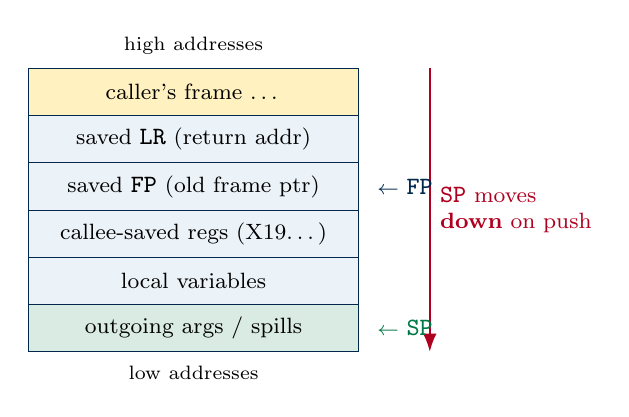
\begin{tikzpicture}[font=\footnotesize]
\tikzset{slot/.style={draw=umblue,minimum width=4.2cm,minimum height=0.6cm,fill=soft}}
\node[slot,fill=maize!25] (a) at (0,4) {caller's frame \dots};
\node[slot] (b) at (0,3.4) {saved \code{LR} (return addr)};
\node[slot] (c) at (0,2.8) {saved \code{FP} (old frame ptr)};
\node[slot] (d) at (0,2.2) {callee-saved regs (X19\dots)};
\node[slot] (e) at (0,1.6) {local variables};
\node[slot,fill=good!15] (f) at (0,1.0) {outgoing args / spills};
\draw[-{Latex},warn,thick] (3.0,4.3) -- (3.0,0.7) node[midway,right,align=left]
   {\code{SP} moves\\\textbf{down} on push};
\node[right=0.1cm of c,font=\scriptsize\color{umblue}] {$\leftarrow$ \code{FP}};
\node[right=0.1cm of f,font=\scriptsize\color{good}] {$\leftarrow$ \code{SP}};
\node[above=0.05cm of a,font=\scriptsize] {high addresses};
\node[below=0.05cm of f,font=\scriptsize] {low addresses};
\end{tikzpicture}
\end{center}

\begin{formbox}[The calling-convention contract]
\textbf{Caller-saved (X9--X15, X0--X7):} if the \emph{caller} needs a value after the call, the
caller must save it first --- the callee may clobber these freely.\\
\textbf{Callee-saved (X19--X28, FP, LR):} if the \emph{callee} wants to use one, it must save the
old value on entry and restore it before returning. The caller sees them unchanged.\\
\textbf{Arguments:} first 8 in \code{X0--X7}; extras on the stack. \textbf{Return value:} \code{X0}.
\textbf{Return address:} \code{BL} puts it in \code{LR}; \code{BR LR} returns.
\end{formbox}

\subsection{Standard function prologue / epilogue}
\begin{multicols}{2}
\textbf{Prologue (on entry):}
\begin{lstlisting}
  SUBI SP, SP, #16     // make frame
  STUR LR,  [SP,#8]    // save return addr
  STUR X19, [SP,#0]    // save callee reg
  ... body ...
\end{lstlisting}
\columnbreak

\textbf{Epilogue (before return):}
\begin{lstlisting}
  LDUR X19, [SP,#0]    // restore
  LDUR LR,  [SP,#8]    // restore ret addr
  ADDI SP, SP, #16     // pop frame
  BR   LR              // return
\end{lstlisting}
\end{multicols}

\begin{pitbox}
For \textbf{recursive} or non-leaf functions you \emph{must} save \code{LR} --- otherwise the
inner \code{BL} overwrites it and you can never return. Leaf functions that make no calls and use
only temporaries may skip the frame entirely.
\end{pitbox}

%==============================================================================
\section{Digital Logic}
%==============================================================================

\subsection{Boolean algebra \& gates}
\begin{multicols}{2}
\begin{itemize}
\item \code{AND} $=A\cdot B$, \code{OR} $=A+B$, \code{NOT}$=\overline{A}$.
\item \code{NAND}$=\overline{A\cdot B}$, \code{NOR}$=\overline{A+B}$, \code{XOR}$=A\oplus B$ (1 iff inputs differ).
\item \textbf{NAND and NOR are universal} --- any function can be built from only NANDs (or only NORs).
\end{itemize}
\columnbreak
\textbf{Key identities}
\begin{itemize}
\item De Morgan: $\overline{A\cdot B}=\overline{A}+\overline{B}$, \;$\overline{A+B}=\overline{A}\cdot\overline{B}$.
\item Distributive: $A(B+C)=AB+AC$.
\item Absorption: $A+AB=A$.
\item $A+\overline{A}=1$,\; $A\cdot\overline{A}=0$.
\end{itemize}
\end{multicols}

\subsection{Combinational building blocks}
\begin{itemize}
\item \textbf{Multiplexer (MUX):} $2^n$ data inputs, $n$ select lines, 1 output. Picks one input.
A 2:1 MUX: $\text{out}=\overline{S}\cdot A + S\cdot B$. \emph{The fundamental ``choose'' element in a datapath.}
\item \textbf{Decoder:} $n$ inputs $\to$ $2^n$ outputs, exactly one hot. Used to select registers / memory rows.
\item \textbf{Adder:} full adder per bit, carry rippling. $\text{Sum}=A\oplus B\oplus C_{in}$,
$C_{out}=AB+(A\oplus B)C_{in}$. Subtraction $=A + \overline{B} + 1$.
\end{itemize}

\subsection{Sum-of-products from a truth table}
\begin{enumerate}
\item Write the truth table for the function.
\item For every row where output $=1$, write an AND term (a \emph{minterm}) of the inputs
(complemented where the input is 0).
\item OR all those minterms. Optionally simplify with Boolean algebra or a Karnaugh map.
\end{enumerate}

\subsection{Sequential logic: state \& clocks}
Combinational logic has no memory; \textbf{sequential} logic stores state.
\begin{itemize}
\item \textbf{D flip-flop:} on the clock edge, captures input \code{D} into output \code{Q} and
holds it until the next edge. The atom of state (registers = arrays of D-FFs).
\item \textbf{Clock period} must exceed the longest combinational path between flip-flops
(plus setup time): $T_{clk} \ge t_{cq}+t_{logic}+t_{setup}$. This is what limits clock speed.
\end{itemize}

\subsection{Finite State Machines (FSM)}
A machine with state registers + combinational ``next-state'' and ``output'' logic.
\begin{center}
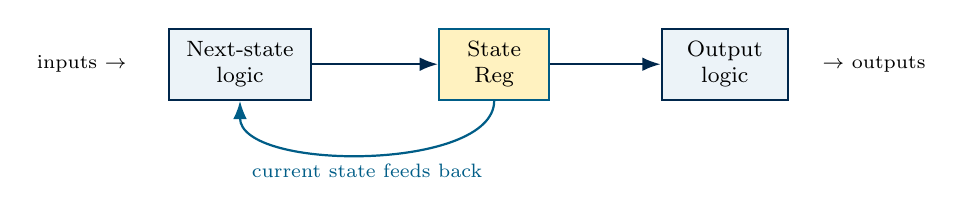
\begin{tikzpicture}[font=\footnotesize,node distance=1.0cm]
\node[draw=umblue,thick,fill=soft,align=center,minimum width=1.8cm,minimum height=0.9cm] (cl) {Next-state\\logic};
\node[draw=accent,thick,fill=maize!25,align=center,right=1.6cm of cl,minimum width=1.4cm,minimum height=0.9cm] (reg) {State\\Reg};
\node[draw=umblue,thick,fill=soft,align=center,right=1.4cm of reg,minimum width=1.6cm,minimum height=0.9cm] (out) {Output\\logic};
\draw[-{Latex},umblue,thick] (cl)--(reg);
\draw[-{Latex},umblue,thick] (reg)--(out);
\draw[-{Latex},accent,thick] (reg.south) .. controls +(0,-0.9) and +(0,-0.9) .. (cl.south)
  node[midway,below,font=\scriptsize]{current state feeds back};
\node[left=0.4cm of cl,font=\scriptsize]{inputs $\rightarrow$};
\node[right=0.3cm of out,font=\scriptsize]{$\rightarrow$ outputs};
\end{tikzpicture}
\end{center}
\textbf{To design one:} (1) draw the state diagram, (2) assign binary codes to states,
(3) build the truth table mapping (current state, input)$\to$(next state, output),
(4) derive logic via sum-of-products. Mealy outputs depend on state+input; Moore on state only.

%==============================================================================
\section{Single-Cycle Datapath}
%==============================================================================

\begin{keybox}[Idea]
Execute one entire instruction every clock cycle. Simple, but the clock must be slow enough for
the \emph{worst-case} instruction (usually \code{lw}, which touches PC, regs, ALU, \emph{and} memory).
\end{keybox}

\subsection{The five things every instruction does}
\textbf{IF} fetch instruction $\to$ \textbf{ID} decode \& read registers $\to$ \textbf{EX}
ALU operation $\to$ \textbf{MEM} access data memory $\to$ \textbf{WB} write result to a register.
Single-cycle does all five in one (long) cycle.

\begin{center}
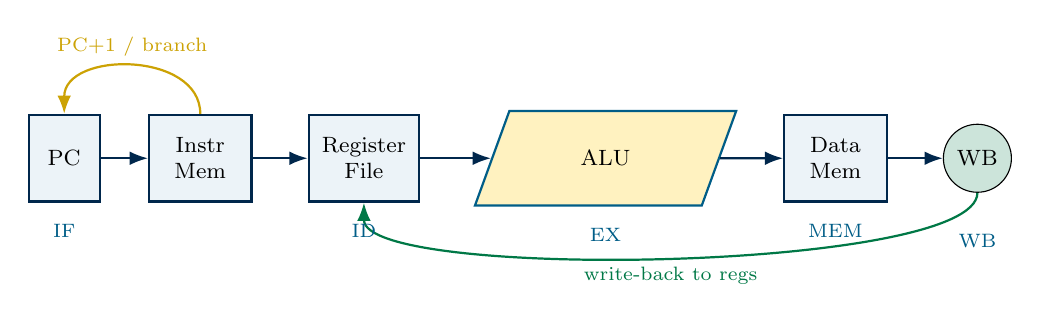
\begin{tikzpicture}[font=\footnotesize,node distance=0.7cm]
\tikzset{u/.style={draw=umblue,thick,fill=soft,minimum height=1.1cm,align=center}}
\node[u,minimum width=0.9cm] (pc) {PC};
\node[u,right=0.6cm of pc,minimum width=1.3cm] (im) {Instr\\Mem};
\node[u,right=0.7cm of im,minimum width=1.4cm] (rf) {Register\\File};
\node[draw=accent,thick,fill=maize!25,right=0.9cm of rf,trapezium,trapezium left angle=70,trapezium right angle=110,minimum height=1.2cm,minimum width=1.1cm] (alu) {ALU};
\node[u,right=0.8cm of alu,minimum width=1.3cm] (dm) {Data\\Mem};
\node[draw,circle,fill=good!20,right=0.7cm of dm,minimum size=0.6cm] (wb) {WB};
\draw[-{Latex},umblue,thick] (pc)--(im);
\draw[-{Latex},umblue,thick] (im)--(rf);
\draw[-{Latex},umblue,thick] (rf)--(alu);
\draw[-{Latex},umblue,thick] (alu)--(dm);
\draw[-{Latex},umblue,thick] (dm)--(wb);
\draw[-{Latex},good,thick] (wb.south) .. controls +(0,-1) and +(0,-1) .. (rf.south)
   node[midway,below,font=\scriptsize]{write-back to regs};
\draw[-{Latex},maize!80!black,thick] (im.north) .. controls +(0,0.8) and +(0,0.8) .. (pc.north)
   node[midway,above,font=\scriptsize]{PC+1 / branch};
\node[below=0.15cm of pc,font=\scriptsize\color{accent}]{IF};
\node[below=0.15cm of rf,font=\scriptsize\color{accent}]{ID};
\node[below=0.15cm of alu,font=\scriptsize\color{accent}]{EX};
\node[below=0.15cm of dm,font=\scriptsize\color{accent}]{MEM};
\node[below=0.4cm of wb,font=\scriptsize\color{accent}]{WB};
\end{tikzpicture}
\end{center}

\textbf{Control signals} (set by the opcode) steer the MUXes: \code{RegWrite}, \code{ALUSrc}
(register vs. sign-extended offset), \code{MemRead}/\code{MemWrite}, \code{MemToReg} (ALU result
vs. loaded data), \code{Branch}, \code{PCSrc}.

%==============================================================================
\section{Multi-Cycle Datapath}
%==============================================================================

\begin{keybox}[Idea]
Break each instruction into several \emph{short} cycles (roughly one per stage). A short clock
period plus reusing hardware (one ALU, one memory) across cycles. Different instructions take
different numbers of cycles (e.g. \code{lw}=5, \code{add}=4, \code{beq}=3).
\end{keybox}
\textbf{Trade-off vs. single-cycle:} clock period set by the \emph{slowest stage}, not the
slowest \emph{instruction}; hardware reused; controlled by an FSM. But more cycles per
instruction and more control complexity. This motivates \textbf{pipelining}: keep the short
cycle, but overlap instructions so you finish (close to) one per cycle.

%==============================================================================
\section{Pipelining}
%==============================================================================

\begin{keybox}[The laundry analogy]
Don't wait for one load of laundry to wash$\to$dry$\to$fold before starting the next. Once the
washer is free, start washing load 2 while load 1 dries. \textbf{Pipelining overlaps the stages
of consecutive instructions.} Latency per instruction stays the same; \emph{throughput} rises to
$\approx$ 1 instruction/cycle.
\end{keybox}

\subsection{The classic 5-stage pipeline}
Stages \textbf{IF, ID, EX, MEM, WB} separated by \textbf{pipeline registers} (IF/ID, ID/EX,
EX/MEM, MEM/WB) that carry each instruction's data and control forward.

\begin{center}
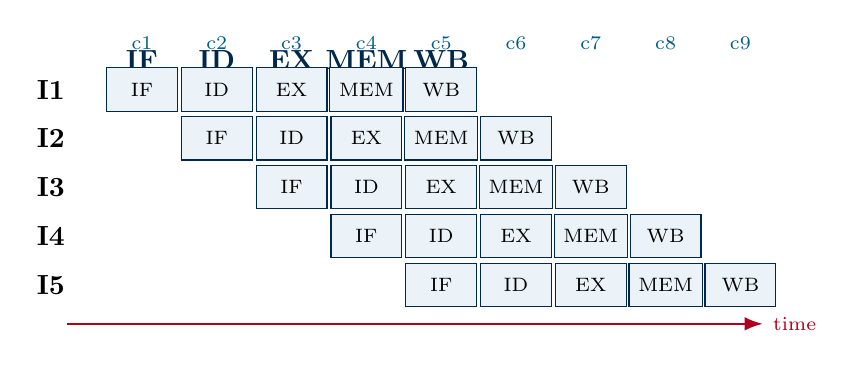
\begin{tikzpicture}[font=\scriptsize,x=0.95cm,y=0.62cm]
\foreach \s [count=\c from 1] in {IF,ID,EX,MEM,WB}
   \node[font=\bfseries\color{umblue}] at (\c+0.5,5.6) {\s};
\foreach \i [count=\r from 0] in {1,2,3,4,5}{
   \node[anchor=east,font=\bfseries] at (0.6,5-\r){I\i};
   \foreach \s [count=\c from 1] in {IF,ID,EX,MEM,WB}{
     \pgfmathtruncatemacro{\x}{\c+\r}
     \node[draw=umblue,fill=soft,minimum width=0.9cm,minimum height=0.55cm] at (\x+0.5,5-\r){\s};
   }
}
\foreach \cyc in {1,...,9}\node[font=\scriptsize\color{accent}] at (\cyc+0.5,5.95){c\cyc};
\draw[-{Latex},warn,thick](0.5,0.2)--(9.8,0.2)node[right]{time};
\end{tikzpicture}
\end{center}
In steady state (cycle~5+), \textbf{five instructions are in flight at once}, one per stage.

\begin{formbox}[Pipeline speedup]
Ideal speedup $\approx$ number of stages. For $N$ instructions on a $k$-stage pipeline:
\[ \text{cycles} = N + (k-1)\quad(\text{the }k-1\text{ is the fill/drain ``startup'').}\]
As $N\to\infty$, CPI $\to 1$. Real speedup is less due to \textbf{hazards}.
\end{formbox}

\subsection{Hazards --- the three reasons pipelines stall}
\begin{enumerate}
\item \textbf{Structural hazard:} two instructions need the same hardware in the same cycle.
Solved by duplicating resources (separate instruction \& data memories; write regs in first half
of a cycle, read in the second).
\item \textbf{Data hazard:} an instruction needs a result that an earlier, still-in-flight
instruction hasn't written back yet.
\item \textbf{Control hazard:} after a branch, we don't yet know which instruction to fetch next.
\end{enumerate}

\subsubsection{Data hazards \& forwarding}
\begin{center}
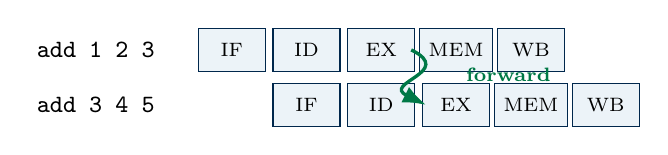
\begin{tikzpicture}[font=\scriptsize,x=0.95cm,y=0.7cm]
\node[anchor=east] at (0.6,2){\code{add 1 2 \textbf{3}}};
\node[anchor=east] at (0.6,1){\code{add \textbf{3} 4 5}};
\foreach \s [count=\c from 1] in {IF,ID,EX,MEM,WB}
   \node[draw=umblue,fill=soft,minimum width=0.85cm,minimum height=0.55cm] at (\c+0.5,2){\s};
\foreach \s [count=\c from 2] in {IF,ID,EX,MEM,WB}
   \node[draw=umblue,fill=soft,minimum width=0.85cm,minimum height=0.55cm] at (\c+0.5,1){\s};
% forward from EX/MEM of I1 to EX of I2
\draw[-{Latex},good,very thick] (3.9,2.0) .. controls +(0.6,-0.4) and +(-0.6,0.4) .. (4.1,1.0);
\node[good,font=\scriptsize\bfseries] at (5.2,1.55){forward};
\end{tikzpicture}
\end{center}
\textbf{Forwarding (bypassing):} route the ALU result directly from a later pipeline register
(EX/MEM or MEM/WB) back into the EX stage's input, instead of waiting for WB. Eliminates most
data-hazard stalls.

\begin{pitbox}[The load-use hazard cannot be fully forwarded]
A \code{lw} produces its value at the end of \textbf{MEM}, but the next instruction needs it in
\textbf{EX} --- one cycle too early. You \emph{must insert one stall (bubble)} (or the compiler
reorders code). After the bubble, forward from MEM/WB.
\end{pitbox}

\subsubsection{Control hazards \& branch handling}
A \code{beq} resolves late (its outcome/target known in EX or MEM). Meanwhile the pipeline keeps
fetching. Solutions:
\begin{itemize}
\item \textbf{Stall} until the branch resolves (simple, slow).
\item \textbf{Predict not-taken}: keep fetching the next sequential instructions; if the branch
\emph{is} taken, \textbf{flush} (squash) the wrongly-fetched instructions (turn them into noops).
\item \textbf{Branch prediction} (dynamic): a predictor (e.g. a 1- or 2-bit saturating counter
per branch) guesses taken/not-taken from history; correct guesses cost nothing, mispredicts pay
the flush penalty.
\item \textbf{Resolve branches earlier} in the pipeline to shrink the penalty.
\end{itemize}

\begin{formbox}[Stall/flush cost]
$\text{Extra cycles} = (\text{\# hazards}) \times (\text{penalty per hazard})$. A branch resolved in
stage $s$ that was predicted wrong flushes $s-1$ instructions $\Rightarrow$ penalty $s-1$ cycles.
\end{formbox}

\subsubsection{Dependency types (know the vocabulary)}
\begin{itemize}
\item \textbf{RAW (Read-After-Write)} --- a \emph{true} dependence: an instruction reads a register a
prior instruction writes. \textbf{This is the only hazard in the LC2K in-order pipeline}, and the one
forwarding fixes.
\item \textbf{WAR / WAW} --- ``false'' (name) dependences that only matter with out-of-order or
register renaming; \textbf{they do not occur} in the simple in-order 5-stage pipeline.
\end{itemize}

\subsubsection{Dynamic branch prediction: the 2-bit saturating counter}
A 1-bit predictor mispredicts \emph{twice} per loop (on the last \emph{and} first iteration). A
\textbf{2-bit} predictor adds hysteresis --- it must be wrong twice in a row to flip its
prediction, so a loop branch mispredicts only once (on loop exit).
\begin{center}
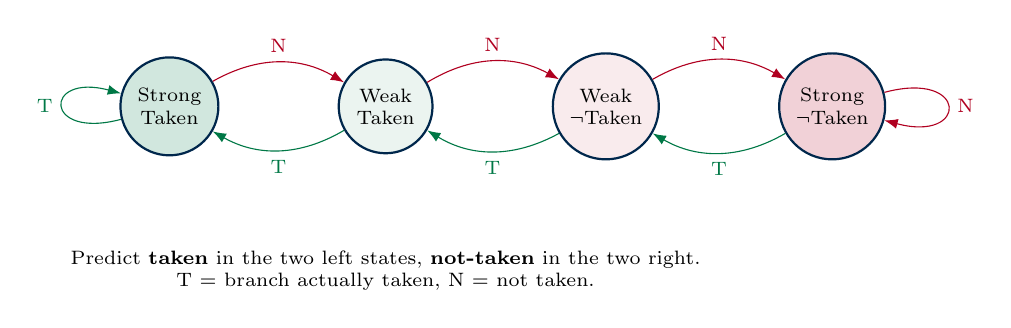
\begin{tikzpicture}[font=\scriptsize,node distance=1.5cm,>=Latex]
\tikzset{st/.style={draw=umblue,thick,circle,minimum size=1.1cm,align=center,fill=soft}}
\node[st,fill=good!18] (st) {Strong\\Taken};
\node[st,fill=good!8,right=of st] (wt) {Weak\\Taken};
\node[st,fill=warn!8,right=of wt] (wn) {Weak\\$\neg$Taken};
\node[st,fill=warn!18,right=of wn] (sn) {Strong\\$\neg$Taken};
\draw[->,good] (st) to[loop left] node[left]{T} ();
\draw[->,warn] (sn) to[loop right] node[right]{N} ();
\draw[->,warn,bend left] (st) to node[above]{N} (wt);
\draw[->,good,bend left] (wt) to node[below]{T} (st);
\draw[->,warn,bend left] (wt) to node[above]{N} (wn);
\draw[->,good,bend left] (wn) to node[below]{T} (wt);
\draw[->,warn,bend left] (wn) to node[above]{N} (sn);
\draw[->,good,bend left] (sn) to node[below]{T} (wn);
\node[below=1.1cm of wt,font=\scriptsize,align=center]
 {Predict \textbf{taken} in the two left states, \textbf{not-taken} in the two right.\\
  T = branch actually taken, N = not taken.};
\end{tikzpicture}
\end{center}

\subsection{The LC2K Pipeline Lab (Project 3) --- implementation cheat sheet}

\begin{keybox}[What Project 3 asks for]
Write a C simulator of the LC2K running on a \textbf{5-stage pipeline} with \textbf{full forwarding},
a \textbf{1-cycle load-use stall}, and \textbf{predict-not-taken} branches resolved in \textbf{MEM}.
Every cycle you advance all five stages ``simultaneously'' and print the state. Correctness ==
your final register/memory values and total cycle count match the reference.
\end{keybox}

\subsubsection{The pipeline-register and machine state structs}
Five pipeline registers sit \emph{between} the stages; each carries the \code{instr} plus whatever
that boundary needs. \textbf{Use the exact structs in the provided starter code} --- the fields below
are the standard set:
\begin{lstlisting}[language=C]
#define NOOPINSTR 0x1c00000   // opcode 111 (noop) in bits 24-22

typedef struct IFIDStruct  { int instr; int pcPlus1; } IFIDType;
typedef struct IDEXStruct  { int instr; int pcPlus1;
                             int readRegA; int readRegB; int offset; } IDEXType;
typedef struct EXMEMStruct { int instr; int branchTarget;
                             int aluResult; int readRegB; } EXMEMType;
typedef struct MEMWBStruct { int instr; int writeData; } MEMWBType;
typedef struct WBENDStruct { int instr; int writeData; } WBENDType;

typedef struct stateStruct {
    int pc;
    int instrMem[NUMMEMORY];  int dataMem[NUMMEMORY];
    int reg[NUMREGS];         int numMemory;
    IFIDType IFID;  IDEXType IDEX;  EXMEMType EXMEM;
    MEMWBType MEMWB; WBENDType WBEND;
    int cycles;               // cycles simulated so far
} stateType;
\end{lstlisting}

\begin{keybox}[The double-buffering rule --- this is THE structural trick]
Keep two copies: \code{state} (this cycle's values, read-only) and \code{newState} (next cycle, you
write it). Each stage \textbf{reads from \code{state} and writes into \code{newState}}. At the end of
the cycle do \code{state = newState}. \textbf{Iron rule:} \code{state} never appears on the
left-hand side of an assignment; \code{newState} never appears on the right. This makes all five
stages update ``at the same clock edge,'' exactly like real hardware.
\end{keybox}

\subsubsection{What each stage does (and which register it writes)}
\begin{center}
\renewcommand{\arraystretch}{1.18}
\begin{tabular}{@{}l p{0.62\textwidth} l@{}}
\toprule
\textbf{Stage} & \textbf{Work (reads \code{state}, writes \code{newState})} & \textbf{Writes}\\
\midrule
IF  & fetch \code{instrMem[pc]}; \code{newState.pc = pc+1}                          & \code{IFID}\\
ID  & decode \code{IFID.instr}; read \code{reg[regA]}, \code{reg[regB]}; sign-extend offset & \code{IDEX}\\
EX  & compute: \code{add/nor} ALU op; \code{lw/sw} address \code{regA+offset}; \code{branchTarget = IDEX.pcPlus1 + offset}; \textbf{apply forwarding here} & \code{EXMEM}\\
MEM & \code{lw}: read \code{dataMem}; \code{sw}: write \code{dataMem}; \textbf{resolve \code{beq}} (taken? squash) & \code{MEMWB}\\
WB  & write \code{reg[dest]} from \code{MEMWB.writeData}                            & \code{WBEND}\\
\bottomrule
\end{tabular}
\end{center}
The extra \textbf{WBEND} register exists \emph{only} so forwarding can reach an instruction three
slots behind (the register-file write effectively lands a cycle ``late'' in this model).

\subsubsection{Forwarding (done entirely in EX) --- the exact algorithm}
For the instruction now in EX, you need up-to-date \code{regA} and \code{regB}. Check the three
older instructions ahead of it and take the value from the \textbf{most recent (closest) producer:}
\begin{formbox}[Forwarding priority: EXMEM $\;>\;$ MEMWB $\;>\;$ WBEND]
For each source register $r$ that EX needs:
\begin{enumerate}
\item if \code{EXMEM} holds an \code{add/nor/lw} whose \textbf{dest} $=r$ $\Rightarrow$ use \code{EXMEM.aluResult} (lw's value isn't ready yet --- see stall below);
\item else if \code{MEMWB} dest $=r$ $\Rightarrow$ use \code{MEMWB.writeData};
\item else if \code{WBEND} dest $=r$ $\Rightarrow$ use \code{WBEND.writeData};
\item else use the value read from the register file (\code{IDEX.readRegA/B}).
\end{enumerate}
\textbf{Check newest first and stop} --- a later write must override an earlier one.
\end{formbox}
\begin{pitbox}[Computing ``dest'' depends on the opcode]
\code{add}/\code{nor} write \textbf{destReg = bits 2--0}. \code{lw} writes \textbf{regB = bits 18--16}.
\code{sw}, \code{beq}, \code{noop}, \code{halt} write \textbf{no register} --- never forward from them.
Compute each producer's destination by reading \emph{its} opcode, not the consumer's.
\end{pitbox}

\subsubsection{The load-use stall (the one case forwarding can't fix)}
\begin{center}
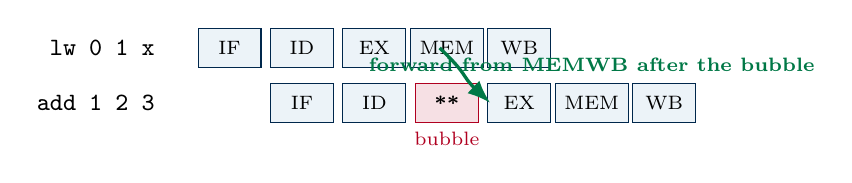
\begin{tikzpicture}[font=\scriptsize,x=0.92cm,y=0.7cm]
\node[anchor=east] at (0.6,2){\code{lw 0 1 x}};
\node[anchor=east] at (0.6,1){\code{add 1 2 3}};
\foreach \s [count=\c from 1] in {IF,ID,EX,MEM,WB}
   \node[draw=umblue,fill=soft,minimum width=0.8cm,minimum height=0.5cm] at (\c+0.5,2){\s};
% dependent: IF ID then a bubble in EX (stall), then EX MEM WB
\node[draw=umblue,fill=soft,minimum width=0.8cm,minimum height=0.5cm] at (2.5,1){IF};
\node[draw=umblue,fill=soft,minimum width=0.8cm,minimum height=0.5cm] at (3.5,1){ID};
\node[draw=warn,fill=warn!12,minimum width=0.8cm,minimum height=0.5cm] at (4.5,1){\textbf{**}};
\node[draw=umblue,fill=soft,minimum width=0.8cm,minimum height=0.5cm] at (5.5,1){EX};
\node[draw=umblue,fill=soft,minimum width=0.8cm,minimum height=0.5cm] at (6.5,1){MEM};
\node[draw=umblue,fill=soft,minimum width=0.8cm,minimum height=0.5cm] at (7.5,1){WB};
\draw[-{Latex},good,very thick] (4.4,2.0) .. controls +(0.4,-0.5) and +(-0.4,0.5) .. (5.1,1.0);
\node[good,font=\scriptsize\bfseries] at (6.5,1.7){forward from MEMWB after the bubble};
\node[warn,font=\scriptsize] at (4.5,0.35){bubble};
\end{tikzpicture}
\end{center}
\textbf{Detect} in the EX stage: if the instruction in \code{IDEX} is a \code{lw} whose dest (regB)
equals \code{regA} or \code{regB} of the instruction currently in \code{IFID}. \textbf{To stall one
cycle:}
\begin{enumerate}
\item \textbf{Do not advance} PC (\code{newState.pc = state.pc}).
\item \textbf{Freeze IFID} (\code{newState.IFID = state.IFID}) --- re-decode the stalled instruction.
\item \textbf{Inject a bubble} into \code{IDEX}: set \code{newState.IDEX.instr = NOOPINSTR}.
\end{enumerate}
Next cycle the dependent instruction reaches EX while the \code{lw} is in MEMWB --- forwarding now works.

\subsubsection{Branch handling: predict-not-taken, resolve in MEM}
\begin{center}
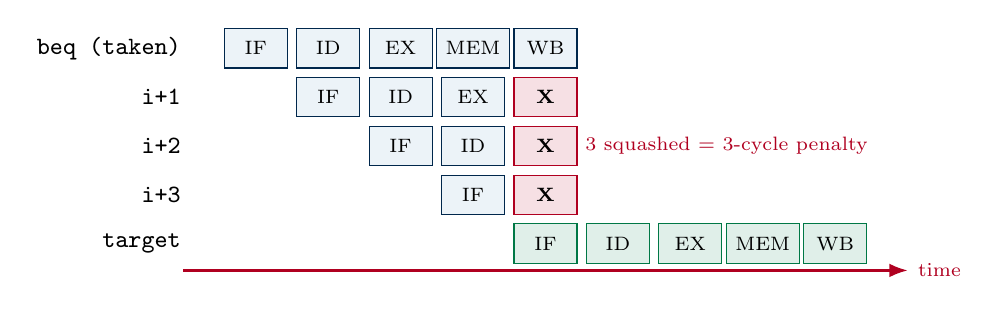
\begin{tikzpicture}[font=\scriptsize,x=0.92cm,y=0.62cm]
\node[anchor=east] at (0.6,4){\code{beq (taken)}};
\node[anchor=east] at (0.6,3){\code{i+1}};
\node[anchor=east] at (0.6,2){\code{i+2}};
\node[anchor=east] at (0.6,1){\code{i+3}};
\node[anchor=east] at (0.6,0){\code{target}};
\foreach \s [count=\c from 1] in {IF,ID,EX,MEM,WB}
   \node[draw=umblue,fill=soft,minimum width=0.8cm,minimum height=0.5cm] at (\c+0.5,4){\s};
% squashed instrs
\foreach \s/\c/\bad in {IF/2/0,ID/3/0,EX/4/0} \node[draw=umblue,fill=soft,minimum width=0.8cm,minimum height=0.5cm] at (\c+0.5,3){\s};
\node[draw=warn,fill=warn!12,minimum width=0.8cm,minimum height=0.5cm] at (5.5,3){\textbf{X}};
\foreach \s/\c in {IF/3,ID/4} \node[draw=umblue,fill=soft,minimum width=0.8cm,minimum height=0.5cm] at (\c+0.5,2){\s};
\node[draw=warn,fill=warn!12,minimum width=0.8cm,minimum height=0.5cm] at (5.5,2){\textbf{X}};
\node[draw=umblue,fill=soft,minimum width=0.8cm,minimum height=0.5cm] at (4.5,1){IF};
\node[draw=warn,fill=warn!12,minimum width=0.8cm,minimum height=0.5cm] at (5.5,1){\textbf{X}};
% target fetched after resolve in MEM (cycle 5)
\foreach \s [count=\c from 5] in {IF,ID,EX,MEM,WB}
   \node[draw=good,fill=good!12,minimum width=0.8cm,minimum height=0.5cm] at (\c+0.5,0){\s};
\node[warn,font=\scriptsize] at (8.0,2){3 squashed = 3-cycle penalty};
\draw[-{Latex},warn,thick](0.5,-0.55)--(10.5,-0.55)node[right]{time};
\end{tikzpicture}
\end{center}
\begin{enumerate}
\item \textbf{Predict not-taken:} IF just keeps fetching \code{pc+1} --- no special action for branches in IF/ID/EX.
\item In \textbf{EX}, still compute \code{branchTarget = IDEX.pcPlus1 + offset} and carry it (plus
whether \code{regA==regB}) into \code{EXMEM}.
\item In \textbf{MEM}, if the \code{beq} is \emph{taken}, you mispredicted: set
\code{newState.pc = EXMEM.branchTarget} and \textbf{squash the 3 younger instructions} by setting
\code{newState.IFID.instr}, \code{newState.IDEX.instr}, and \code{newState.EXMEM.instr} to
\code{NOOPINSTR}.
\end{enumerate}
\textbf{Penalty = 3 cycles per taken branch} (since resolution is in MEM, stage~4, $\Rightarrow 4-1=3$).
A not-taken branch costs nothing.

\subsubsection{Per-cycle driver \& start/stop}
\begin{enumerate}
\item Init: \code{pc=0}, all five pipeline-register \code{instr} fields $=$ \code{NOOPINSTR}, \code{cycles=0}.
\item Each iteration: \code{printState(\&state)} \emph{first}, then compute WB$\to$MEM$\to$EX$\to$ID$\to$IF
into \code{newState} (any stage order is fine since you only read \code{state}), apply stall/squash, then \code{state = newState}, \code{state.cycles++}.
\item \textbf{Halt} when the instruction reaching the \textbf{MEM} (some specs say WB) stage is
\code{halt}: print the final state and stop. Do \emph{not} halt the moment you fetch it --- let it flow down the pipe.
\end{enumerate}

\begin{pitbox}[Project 3 bugs that cost the most points]
1. Forwarding from a \code{sw}/\code{beq} (they write no register). 2. Wrong dest field
(\code{add}=bits 2--0 vs \code{lw}=bits 18--16). 3. Checking forwarding \emph{oldest}-first so an
older value wrongly wins --- go newest (EXMEM) first. 4. Forgetting to also freeze \code{IFID} and
hold \code{pc} on a load-use stall (you get a bubble but lose the instruction). 5. Off-by-one on
\code{branchTarget} --- it is \code{pcPlus1 + offset}, \emph{not} \code{pc + offset}. 6. Halting on
fetch instead of letting \code{halt} drain to the end. 7. Writing to \code{state} instead of
\code{newState} (stages stop being simultaneous).
\end{pitbox}

%==============================================================================
\section{Performance Analysis}
%==============================================================================

\begin{formbox}[The Iron Law of performance]
\[
\text{CPU time} \;=\; \underbrace{\text{Instructions}}_{\text{program/ISA/compiler}}
\times \underbrace{\text{CPI}}_{\text{architecture}}
\times \underbrace{\text{Clock cycle time}}_{\text{technology}}
\;=\; \frac{\text{Instructions}\times\text{CPI}}{\text{Clock rate}}
\]
\end{formbox}

\begin{itemize}
\item \textbf{CPI} = cycles per instruction (average). \textbf{Average CPI} $=\sum_i (\text{freq}_i \times \text{CPI}_i)$.
\item \textbf{Speedup} $= \dfrac{\text{time}_{\text{old}}}{\text{time}_{\text{new}}}$. ($>1$ means faster.)
\item \textbf{MIPS} $= \dfrac{\text{Instruction count}}{\text{exec time}\times 10^6}$ (a flawed metric across ISAs).
\end{itemize}

\begin{formbox}[Amdahl's Law --- the ``speed limit'' of optimization]
If a fraction $f$ of execution is sped up by factor $s$:
\[ \text{Speedup}_{\text{overall}} = \frac{1}{(1-f) + \dfrac{f}{s}} \]
As $s\to\infty$, speedup $\to \dfrac{1}{1-f}$. \textbf{Make the common case fast}: optimizing a
tiny fraction $f$ can never help more than $1/(1-f)$.
\end{formbox}

\textbf{Worked example:} 40\% of a program is parallelizable ($f{=}0.4$) and you speed that part
up $4\times$ ($s{=}4$). Overall speedup $= \frac{1}{0.6 + 0.4/4}=\frac{1}{0.7}\approx 1.43\times$.
Even with $s=\infty$ the cap is $1/0.6\approx1.67\times$.

%==============================================================================
\section{Caches \& the Memory Hierarchy}
%==============================================================================

\begin{keybox}[Why caches exist]
DRAM is huge but slow ($\sim$100s of cycles); registers are fast but tiny. A \textbf{cache} is a
small fast SRAM holding recently/likely-used data. It works because of \textbf{locality}:\\
\textbf{Temporal:} data used now is likely used again soon (loops, variables).\\
\textbf{Spatial:} data near recently-used data is likely used soon (arrays, code). $\Rightarrow$
fetch a whole \textbf{block} (line) at a time.
\end{keybox}

\subsection{Address breakdown}
Every address is split into three fields (sizes depend on cache geometry):
\begin{center}
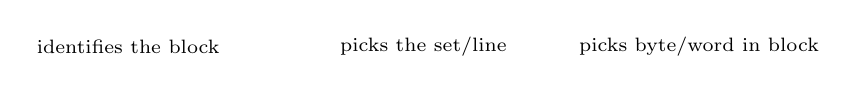
\begin{tikzpicture}[font=\footnotesize]
\field{0}{4}{TAG}{maize!40}
\field{4}{7.5}{INDEX}{accent!20}
\field{7.5}{11}{BLOCK OFFSET}{good!20}
\node[font=\scriptsize] at (2,1.2){identifies the block};
\node[font=\scriptsize] at (5.75,1.2){picks the set/line};
\node[font=\scriptsize] at (9.25,1.2){picks byte/word in block};
\end{tikzpicture}
\end{center}

\begin{formbox}[The bit-counting recipe (do this every cache problem)]
Let block size $=2^b$ bytes, number of sets $=2^s$, address $=m$ bits.
\[
\text{offset bits}=b=\log_2(\text{block size}),\quad
\text{index bits}=s=\log_2(\text{\# sets}),
\]
\[
\text{tag bits}=m-s-b,\qquad
\#\text{sets}=\frac{\text{cache size}}{(\text{block size})\times(\text{associativity})}.
\]
\end{formbox}

\subsection{Mapping: direct, set-associative, fully associative}
\begin{center}
\renewcommand{\arraystretch}{1.2}
\begin{tabular}{@{}l l l@{}}
\toprule
\textbf{Type} & \textbf{A block can go\dots} & \textbf{\# sets / ways}\\
\midrule
Direct-mapped         & in exactly \textbf{1} line (set)           & sets $=$ lines, 1 way\\
$n$-way set-assoc.    & in any of \textbf{$n$} lines of its set     & sets $=$ lines$/n$\\
Fully associative     & in \textbf{any} line                       & 1 set, all ways\\
\bottomrule
\end{tabular}
\end{center}
More associativity $\Rightarrow$ fewer conflict misses but more comparators and slower hits.

\begin{center}
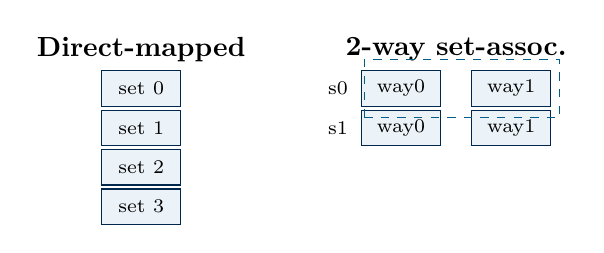
\begin{tikzpicture}[font=\scriptsize,node distance=0.2cm]
\tikzset{ln/.style={draw=umblue,minimum width=1.0cm,minimum height=0.45cm,fill=soft}}
% direct mapped
\node[font=\bfseries] at (1.0,2.6){Direct-mapped};
\foreach \i in {0,1,2,3}\node[ln] at (1.0,2.1-\i*0.5){set \i};
% 2-way
\node[font=\bfseries] at (5.0,2.6){2-way set-assoc.};
\foreach \i in {0,1}{
  \node[ln] at (4.3,2.1-\i*0.5){way0};
  \node[ln] at (5.7,2.1-\i*0.5){way1};
  \node[left=0.05cm of {(3.8,2.1-\i*0.5)},font=\scriptsize] at (3.8,2.1-\i*0.5){s\i};
}
\node[draw=accent,dashed,fit={(3.95,1.85)(6.2,2.35)}]{};
\end{tikzpicture}
\end{center}

\subsection{The 3 C's --- classify every miss}
\begin{itemize}
\item \textbf{Compulsory (cold):} first-ever access to a block. Unavoidable except by prefetching /
bigger blocks.
\item \textbf{Capacity:} cache simply can't hold the working set. Fixed only by a bigger cache.
\item \textbf{Conflict:} block was evicted because too many blocks map to the same set (would have
hit in a fully-associative cache). Fixed by more associativity.
\end{itemize}

\subsection{Replacement \& write policies}
\textbf{Replacement} (which line to evict in an associative set): \textbf{LRU} (least recently
used), FIFO, or random.\\
\textbf{On a write hit:} \emph{Write-through} (update cache \emph{and} memory; simple, more
traffic --- usually with a write buffer) vs. \emph{Write-back} (update cache only, set a
\textbf{dirty bit}; write to memory on eviction; less traffic).\\
\textbf{On a write miss:} \emph{Write-allocate} (load block into cache, then write) --- pairs with
write-back; vs. \emph{No-write-allocate} (write straight to memory) --- pairs with write-through.

\subsection{Performance: AMAT}
\begin{formbox}[Average Memory Access Time]
\[ \text{AMAT} = \text{Hit time} + \text{Miss rate}\times\text{Miss penalty} \]
For multi-level caches, recurse on the miss penalty:
\[ \text{AMAT} = HT_{L1} + MR_{L1}\big(HT_{L2} + MR_{L2}\times MP_{L2}\big) \]
\textbf{Local miss rate} = misses in this level / accesses to this level. \textbf{Global miss
rate} = misses in this level / \emph{total} CPU accesses.
\end{formbox}

\textbf{Worked example:} hit time 1 cycle, miss rate 5\%, miss penalty 100 cycles.
$\text{AMAT}=1+0.05\times100=6$ cycles. Cut miss rate to 2\%: $1+0.02\times100=3$ cycles
($2\times$ faster memory access).

\begin{tipbox}[Cache-aware programming]
Loop over arrays in \textbf{memory order} (row-major in C: vary the \emph{last} index in the
inner loop) to exploit spatial locality. Blocking/tiling keeps a working set inside the cache to
exploit temporal locality. This is the ``performance optimization'' the course rewards.
\end{tipbox}

%==============================================================================
\section{Virtual Memory}
%==============================================================================

\begin{keybox}[Why virtual memory]
Give every process its own private, contiguous-looking address space that's larger than physical
RAM, with \textbf{protection} (processes can't touch each other's memory) and
\textbf{relocation} (programs don't care where they physically land). The OS + hardware translate
\textbf{virtual addresses} $\to$ \textbf{physical addresses}, paging data to/from disk on demand.
\end{keybox}

\subsection{Paging and address translation}
Memory is divided into fixed-size \textbf{pages} (virtual) and \textbf{frames} (physical), e.g.\
4\,KB. A virtual address splits into a \textbf{Virtual Page Number (VPN)} + \textbf{page offset};
the offset is unchanged by translation.

\begin{center}
\begin{tikzpicture}[font=\footnotesize]
\field{0}{5}{Virtual Page Number (VPN)}{accent!20}
\field{5}{8}{page offset}{good!20}
\node at (3.9,-0.6){\textbf{translate}};
\draw[-{Latex},umblue,thick](2.5,-0.15)--(2.5,-1.0);
\begin{scope}[yshift=-1.9cm]
\field{0}{5}{Physical Frame Number (PFN)}{maize!40}
\field{5}{8}{page offset (same)}{good!20}
\end{scope}
\node[right=0.2cm,font=\scriptsize] at (8,0.45){VPN $\to$ PFN via \textbf{page table}};
\node[right=0.2cm,font=\scriptsize] at (8,-1.45){offset copied unchanged};
\end{tikzpicture}
\end{center}

\begin{formbox}[Translation arithmetic]
\[
\text{offset bits} = \log_2(\text{page size}),\quad
\#\text{virtual pages} = \frac{\text{virtual addr space}}{\text{page size}},
\]
\[
\text{PFN bits} = \log_2\!\Big(\frac{\text{physical mem}}{\text{page size}}\Big),\qquad
\text{Physical addr} = \text{PFN}\,\Vert\,\text{offset}.
\]
\end{formbox}

\subsection{Page table}
A per-process table mapping VPN $\to$ PFN, with \textbf{valid}, \textbf{dirty}, \textbf{protection}
bits. Lives in memory. If \code{valid=0} on access $\Rightarrow$ \textbf{page fault}: OS fetches
the page from disk (very slow), updates the table, resumes.

\textbf{Multi-level page tables:} a single flat table for a 64-bit space would be enormous, so use
a tree --- the VPN is split into several indices, each indexing the next-level table. Only tables
for in-use regions exist, saving space (at the cost of multiple memory lookups per translation).

\subsection{TLB --- making translation fast}
\begin{keybox}
A naive load now costs \emph{two} memory accesses (page table, then data). The \textbf{TLB
(Translation Lookaside Buffer)} is a small fast cache of recent VPN$\to$PFN translations.
TLB hit $\Rightarrow$ translate in $\sim$1 cycle.
\end{keybox}

\begin{center}
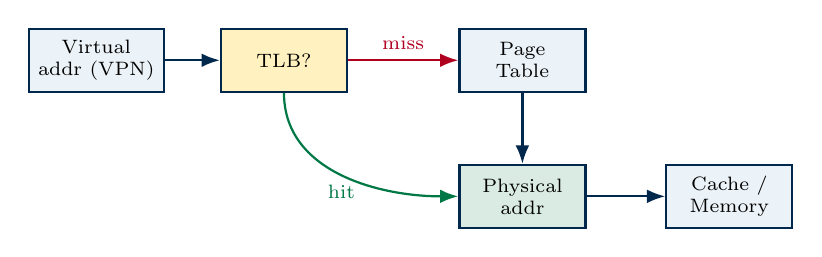
\begin{tikzpicture}[font=\scriptsize,node distance=0.7cm]
\tikzset{b/.style={draw=umblue,thick,fill=soft,minimum width=1.6cm,minimum height=0.8cm,align=center}}
\node[b] (va) {Virtual\\addr (VPN)};
\node[b,right=of va,fill=maize!25] (tlb) {TLB?};
\node[b,right=1.4cm of tlb] (pt) {Page\\Table};
\node[b,below=0.9cm of pt,fill=good!15] (pa) {Physical\\addr};
\node[b,right=1.0cm of pa] (cache) {Cache /\\Memory};
\draw[-{Latex},umblue,thick](va)--(tlb);
\draw[-{Latex},good,thick](tlb) to[out=-90,in=180] node[below,font=\scriptsize]{hit}(pa);
\draw[-{Latex},warn,thick](tlb)--(pt) node[midway,above,font=\scriptsize]{miss};
\draw[-{Latex},umblue,thick](pt)--(pa);
\draw[-{Latex},umblue,thick](pa)--(cache);
\end{tikzpicture}
\end{center}

\textbf{Full access sequence for a load:} (1) check \textbf{TLB} for VPN. (2) TLB miss $\to$ walk
the \textbf{page table} (and on \code{valid=0}, take a \textbf{page fault} to disk). (3) form the
physical address. (4) look it up in the \textbf{cache}; on a cache miss, go to memory.
So three nested ``maybe-miss'' structures: \textbf{TLB $\to$ page table $\to$ cache}.

%==============================================================================
\section{Rapid-Fire Exam Checklists}
%==============================================================================

\begin{tipbox}[LC2K assembly problem]
1. Remember \code{r0}$=0$ by convention. 2. No \code{addi}/immediate-load --- use \code{.fill} +
\code{lw}. 3. \code{beq} offset $=$ targetAddr $-$ (beqAddr$+1$). 4. Negate via \code{nor}+add 1.
5. Each line $=$ one word $=$ one address.
\end{tipbox}

\begin{tipbox}[Pipeline / hazard problem]
1. Draw the cycle-by-cycle diagram. 2. Mark every RAW dependency between in-flight instructions.
3. Can forwarding fix it? (Yes, except load-use $\to$ 1 stall.) 4. Branch: add flush penalty
$=$ (resolve stage $-1$). 5. Total cycles $= N + (k-1) + $ stalls $+$ flushes.
\end{tipbox}

\begin{tipbox}[Cache problem]
1. offset $=\log_2$(block), index $=\log_2$(\# sets), tag $=$ rest. 2. \# sets $=$ size /
(block $\times$ assoc). 3. Trace each access; classify miss as compulsory/capacity/conflict.
4. AMAT $=$ hit $+$ missrate $\times$ penalty. 5. Don't forget valid/dirty/tag \textbf{overhead bits}.
\end{tipbox}

\begin{tipbox}[Virtual memory problem]
1. offset $=\log_2$(page size). 2. VPN bits $=$ virtAddrBits $-$ offset. 3. PFN bits from physical
size. 4. Page-table entries $= 2^{\text{VPN bits}}$ per level. 5. Access path:
TLB $\to$ page table $\to$ cache $\to$ memory.
\end{tipbox}

\begin{center}
\vspace{0.4cm}
{\color{umblue}\rule{\textwidth}{2pt}}\\[4pt]
{\small\itshape End of cheat sheet --- Go Blue. Always re-verify exact opcodes / bit ranges and
the current term's policies against the official EECS 370 spec before your exam.}
\end{center}

\end{document}
